\documentclass[10pt,twocolumn]{article}

\setlength{\marginparwidth}{2cm}

\usepackage{graphicx}
\usepackage[colorlinks=true,allcolors=blue]{hyperref}
\usepackage{todonotes}

\begin{document}

\title{Next-generation design tools for intelligent transportation systems}
\author{Dominik Ascher and Georg Hackenberg}
\maketitle

\begin{abstract}
    \textcolor{red}{TODO}
\end{abstract}

\section{Introduction}
\label{sec:introduction}

The transformative patterns of future mobility are enabled by interconnected and integrated systems and services.
As such, Intelligent Transportation Systems (ITS) establish new transportation paradigms such as connected and autonomous vehicles (CAV), multi-modal and demand-responsive transport systems, and facilitate the transportation electrification by efficient operation of electric vehicles. For this, complex scenarios and their encoded requirements need to be holistically addressed, from which integrated system designs have to be derived, which allow transport infrastructures and their heterogenous actors to be more efficient and sustainable.

Therefore, constituent systems need to be designed with respect to most efficient structures and control strategies within themselves, while accounting for and exploiting the emergent properties they achieve in conjunction and interdependence with other systems, as composed, integrated system-of-systems (SoS). To systematically support the aforementioned systems engineering task, model- and simulation-based systems engineering~\cite{gianni2014modeling} can be employed for abstraction of design problems through the use of system models and their evaluation, i.e. their numerical approximation in terms of concrete behavior at run time. For this, well-defined system models are formulated at design time, for which then simulation aids projecting run-time information and performance metrics about the system under design and its environment. 
However, as systems and their underlying requirements are typically imperfectly understood at the beginning of the design task, methods and tools are needed to explore the possible design space, which support evaluation of system design alternatives and verification of intended system properties. 

%As an effect of underspecified requirements, system models are often not completely understood, and modeling uncertainties need be adressed. 

%Both structural as well as behavioral system design tasks can be supported using an overarching system design methodology at design time as well as at run time. 
%In terms of benefits, on the one hand side, system models faciliate gaining improved system understanding through specification, while allowing rapid system modification through defined variation points for designing a system. On the other hand side, simulation aids approximating information about the system dynamics and performance of a system under design.

For this, in previous work, we established an integrated systems modeling technique for integrated transportation and power systems. Here, our systems modeling technique allows one to model both transportation and power system scenarios, as well as mobility-on-demand scenarios to assess system design options systematically and improving system understanding holistically, based on a formal foundation~\cite{ascher_hackenberg_2014,ascher_hackenberg_2015,ascher_hackenberg_2016,ascher_hackenberg_2017}. The formal foundation was extended by a discrete event formalism \cite{ascher2023discrete} as well as integration with state-of-the-art simulators and predictive models for control strategy optimization \cite{ascher_hackenberg_albayrak_2023}.

\paragraph{Research objective}

With our research, we want to help improve the efficiency and effectiveness of today's transportation systems.
To achieve this goal, we work on methodologies for designing such systems and verifying their properties.
Fundamentally, we promote a formal approach capturing the relevant design decisions and their relations.
Furthermore, we integrate scenario-based simulation of system dynamics and evaluation of emergent properties.
Finally, we exploit optimization algorithms for optimizing system dynamics as well as static design decisions.

\paragraph{Research question}

In this paper, we ask how the next generation of design tools for intelligent transportation systems should look like.
Therefore, first we want to understand which system properties and design decisions should be represented in these tools.
Then, we want to learn how the design decisions could be verified with respect to the desired system properties.
Finally, we want to study how the relevant design information could be represented in a graphical user interface.

\paragraph{Research methodology}

In the following, we first propose a modeling and simulation framework for capturing design decisions and evaluating emergent properties in Section~\ref{sec:approach}.
%Then, we propose a graphical user interface for building system designs, starting simulation runs, and visualizing simulation outcomes in Section~\ref{sec:gui}.
\textcolor{red}{Thereafter, we propose two specific applications of our modeling and simulation framework as well as user interface technology in Section~\ref{sec:application}.}
Finally, we draw our conclusions and describe future direction of research and development on the design of ITS in Section~\ref{sec:conclusion}. 

\section{General approach}
\label{sec:approach}

In this section, we propose a modeling and simulation framework for the design of intelligent transportation systems.
We first introduce the scope and intended usage of the framework in Section ~\ref{sec:scope}.
Secondly, we present the methodology for describing design decisions in Section~\ref{sec:methodology}.
Thirdly, we describe the domain-specific concepts our modeling and simulation framework employs for designs in Section~\ref{sec:domain-specific-modeling}.
%Then, we propose an interface for implementing and integrating custom control strategies in Section~\ref{sec:controller-interface}.
%Finally, we define an interface for collecting statistics during simulation of system dynamics in Section~\ref{sec:statistics-interface}.

\subsection{Intended usage}
\label{sec:scope}

Our underlying modeling technique is based on integrated transportation system modeling techniques, which allow assessment of integrated, electrified ITS systems for the purpose of designing emergent integrated system properties.
In terms of considered domain problems, for instance, future transportation electrification as well as demand-responsive transport scenarios may be investigated.
In terms of use-cases, our modeling technique supports both transportation system and control strategy design.
For instance, transportation engineers may be supported by investigation of transportation infrastructure properties.
On the other hand side, mobility and vehicle fleet operators may be supported by deriving control strategies in the context of on-demand transportation problems.

% \begin{itemize}
% 	\item Transportation System Engineer
 %	\item Mobility Provider
% \end{itemize}

\subsection{Design methodology}
\label{sec:methodology}

Our approach employs model- and simulation-based systems engineering~\cite{gianni2014modeling} for decision-making with respect to system designs for the ITS domain.
Models are described based on the problem domain, where simulation aids obtaining information about and shaping designs of the solution domain.

% TODO Figure
\begin{figure}[!ht]
	\centering
	\missingfigure[figwidth=\columnwidth, figheight=0.7\columnwidth]{Static/dynamic/mixed property optimization}
	\caption{System design methodology}
	\label{fig:concept}
\end{figure}

For system models, each concept is described in terms of their static (i.e.\ time-independent) properties and calculations as well as their dynamic (i.e.\ time-dependent) properties concerning state evolution during simulation including states and actions.
As simulation complexity increases with the number and dimensionality of considered parameters, states, and actions of modeled systems, Discrete-Event Simulation (DES)~\cite{fishman2001discrete} is employed, where events are defined as functions over a system's trajectory of states, which indicate when actions need to be taken in the system simulation.
Thus, simulation complexity is reduced by limiting action space dimensionality and by abstracting from discrete-time resolutions~\cite{ascher2023discrete}.

%Each concept is described in terms of their static (i.e.\ time-independent) properties and calculations as well as their dynamic (i.e.\ time-dependent) state functions typically sampled during computer simulations. In addition, we define events as functions over a system's trajectory of states, which precisely indicate when actions need to be taken in the system simulation. Thus, events significantly reduce simulation complexity by limiting action space dimensionality and by abstracting from discrete-time resolutions. 

Based on the concepts, our approach supports different design tasks, where evaluation of designs is performed using approximate and heuristic optimization techniques. We utilize optimization to evaluate solutions for the following design problems:

\begin{itemize}
    \item \textbf{Static property optimization} concerns static design decisions such as optimization of transportation infrastructure properties.
    \item \textbf{Dynamic property optimization} concerns dynamic design decisions, i.e. optimization of control strategies such as efficient transportation entity behavior.
    \item \textbf{Mixed property optimization} concerns the integrated design task for optimization of both static and dynamic design decisions.
\end{itemize}

%In addition, relationships between components can be incorporated by specifying well-defined component interfaces and their connection.

%\subsubsection{System Theory}
%\label{sec:system-theory}

\subsection{System theory}
\label{sec:domain-specific-modeling}

%Figure~\ref{fig:modeling-technique} provides an overview of main domain concepts, where the formalism is intended to capture a concise and an essential set of static properties, static calculations, and dynamic states as well as events for establishing sound models and control strategies for on-demand transportation systems. For details on the underlying modeling concepts, we refer to \cite{ascher2023discrete}. Subsequently, we describe a brief overview of these concepts.

On a domain-specific modeling level, the approach allows modeling integrated transportation system problems on mesoscopic to microscopic levels, \cite{ascher_hackenberg_2014, ascher_hackenberg_2015}, supported by a formal systems modeling foundation \cite{ascher_hackenberg_2016, ascher_hackenberg_2017} (See Section  \ref{sec:scope}).
Figure \ref{fig:domain-specific-modeling} shows an overview of the domain-specific modeling concepts.

% TODO Figure
\begin{figure}[!ht]
	\centering
	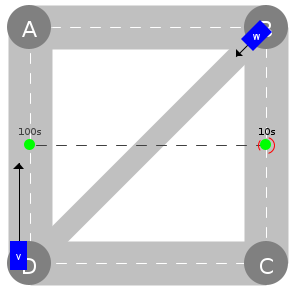
\includegraphics[width=0.6\columnwidth]{../../events/demand.png}
	\caption{Domain-specific modeling concepts.}
	\label{fig:domain-specific-modeling}
\end{figure}

\paragraph{Concepts}

Considered domain concepts for the formalism include intersections $i \in I$, segments $s \in S$ as well as locations $l \in L$ for describing properties about the transportation infrastructure.
Based on the transportation infrastructure, we use charging stations $cs \in CS$ for describing the charging infrastructure. In addition, we describe transportation demands $d \in D$ on the transportation infrastructure.
Finally, we use vehicles $v \in V$ for describing transportation supply and capacities.

\paragraph{States}

\textcolor{red}{TODO}

\paragraph{Events}

\textcolor{red}{TODO}

\paragraph{Constraints}

\textcolor{red}{TODO}

\section{Tool prototype}
\label{sec:tool-prototype}

Based on the general approach explained in Section~\ref{sec:approach} we started developing an open source tool prototype hosted on GitHub\footnote{\url{https://github.com/ghackenberg/transport-ide}}.
The tool prototype is written in Java\footnote{\url{https://docs.oracle.com/javase/tutorial/java/}} and uses the Swing library\footnote{\url{https://docs.oracle.com/javase/tutorial/uiswing/}} as well as the JFreeChart library\footnote{\url{https://www.jfree.org/jfreechart/}} for visualization.
Furthermore, the prototype uses the JGraphT\footnote{\url{https://jgrapht.org/}} library for computing shortest paths in the road network.

In the following, we explain several interesting aspects of the tool prototype:
In Section~\ref{sec:data-model} we dive into the core data structures for representing both static system configurations as well as dynamic system states.
Then, in Section~\ref{sec:controller-interface} we explain how the users can implement and integrate different control strategies into the tool prototype.
Next, in Section~\ref{sec:statistics-interface} we describe the data, which is collected during simulation runs and which can be used for visualizations and possibly training.
Thereafter, in Section~\ref{sec:simulation-engine} we provide an overview of the engine, which computes the discrete events and updates the system states accordingly.
Finally, in Section~\ref{sec:application} we highlight two different applications, which we have implemented already based on the previous framework elements.

%Figure~\ref{fig:software-architecture} illustrates the module architecture of the tool prototype.
%The architecture consists of the eight modules \texttt{model}, \texttt{controller}, \texttt{statistics}, and \texttt{simulator} as well as \texttt{parser}, \texttt{exporter}, \texttt{viewer}, and \texttt{program}.

%\begin{figure}[!ht]
%    \centering
%    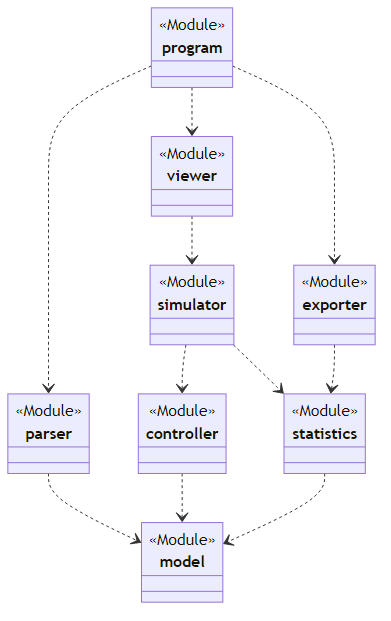
\includegraphics[scale=0.4]{../../diagrams/architecture-v2.png}
%    \caption{Modular software architecture.}
%    \label{fig:software-architecture}
%\end{figure}

%In the following, we discuss each module in more detail including their resposibilities and dependencies on the other modules.

\subsection{Data structures}
\label{sec:data-model}

The \texttt{model} module provides the core data structures for modeling static system configurations and representing dynamic system states.
Figure~\ref{fig:data-model} shows the classes, their attributes, and their relationships.

\begin{figure}[!ht]
    \centering
    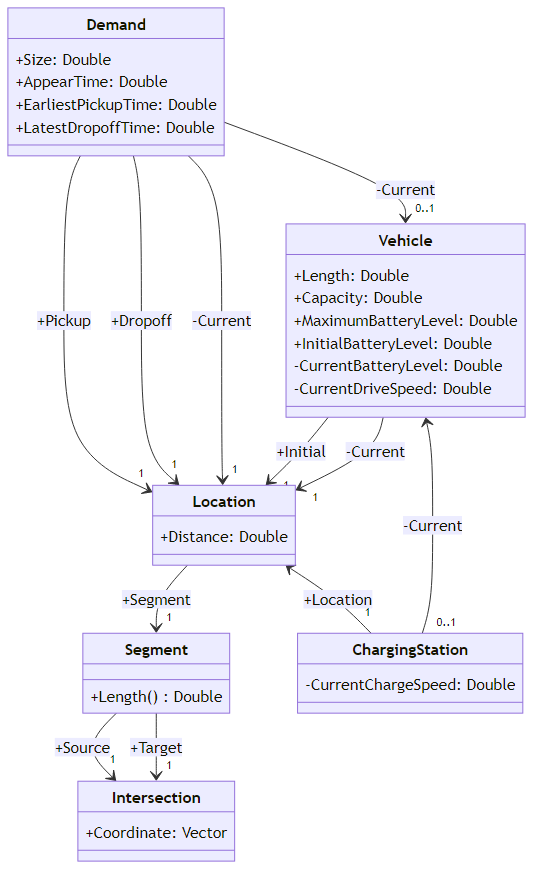
\includegraphics[scale=0.4]{../../diagrams/model/classes-v0.2.png}
    \caption{Configuration and simulation data model.}
    \label{fig:data-model}
\end{figure}

The \texttt{Intersection} class represents intersections of the driving infrastructure.
Each intersection stores its coordinate in three-dimensional space.
Note that we use Cartesian coordinates for simplicity.

The \texttt{Segment} class represents road segments of the driving infrastructure.
Each segment points to its source and its target intersection.
Furthermore, each segment provides a method for computing its length.
Note that we use the Euclidean distance between source and target intersection here.

The \texttt{Location} class represents specific points on the segments of the driving infrastructure.
Each location points to the corresponding segment of the driving infrastructure.
Furthermore, each location stores a distance on this segment.
The distance is measured in Eclidean units of the Cartesian space.

The \texttt{ChargingStation} class represents the charging infrastructure.
Each charging station stores its location on the driving infrastructure.
Furthermore, each charging station optionally points to a current vehicle.
Then, each charging station provides the current charging speed.
Note that the simulator computes the current charging speed dynamically.

The \texttt{Vehicle} class represents the driving resources.
Each vehicle provides an initial and a current location on the driving infrastructure.
The initial location defines the position of the vehicle in the initial state of the simulation.
Then, the simulator continuously updates the current location of the vehicle.
Furthermore, each vehicle stores a length and a capacity, a maximum, an initial, and a current battery level, and a current drive speed.
The length determines how much space the vehicle occupies on the driving infrastructure.
The capacity defines how much demand the vehicle can carry.
The maximum battery level specifies the size of the energy storage.
And the initial battery level stores the load state of the enery storage at simulation start.
Finally, the simulator continuously updates the current battery level as well as the current drive speed.

The \texttt{Demand} class represents the transportation loads to be served.
Each demand points to a pickup and a dropoff location as well as a current location and vehicle.
Furthermore, each demand stores a size as well as an appear, and earliest pickup, and a latest dropoff time.
The simulator continously updates the current location and vehicle.

\subsection{Control strategies}
\label{sec:controller-interface}

%For evaluation of defined system designs, the approach offers an controller interface for defining control strategies. 

During a simulation run, a number of control decisions have to be taken.
For example, when arriving at an intersection each vehicle has to select the next outgoing road segment.
Similarly, when arriving at a demand pickup location each vehicle as to decide whether to serve the demand or not.
The overall system performance heavily depends on the optimality of the individual choices made during a simulation run.
Therefore, one key engineering task for this class of systems is to develop an appropriate control strategy.
Since the desired control strategy cannot be hardcoded upfront, the simulator supports plugging in and testing different strategies.
Each control strategy must implement the controller interface methods depicted in Figure~\ref{fig:controller-interface}.

\begin{figure}[!ht]
    \centering
    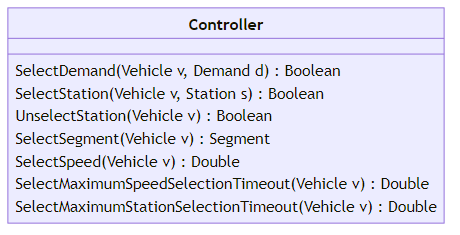
\includegraphics[scale=0.4]{../../diagrams/controller/classes-minimal.png}
    \caption{Methods of the controller interface.}
    \label{fig:controller-interface}
\end{figure}

For tool demonstration and evaluation purposes, we currently provide four different implementations of the controller interface: A \textbf{manual}, a \textbf{random}, a \textbf{greedy}, and a \textbf{smart} control strategy.
Figure~\ref{fig:control-strategies} provides an overview of the four control strategies and their decision logic.
The columns of the matrix represent the individual control strategies, the rows represent the decisions to be taken, and the cells represent the corresponding logic.

\begin{figure}[!ht]
    \centering
    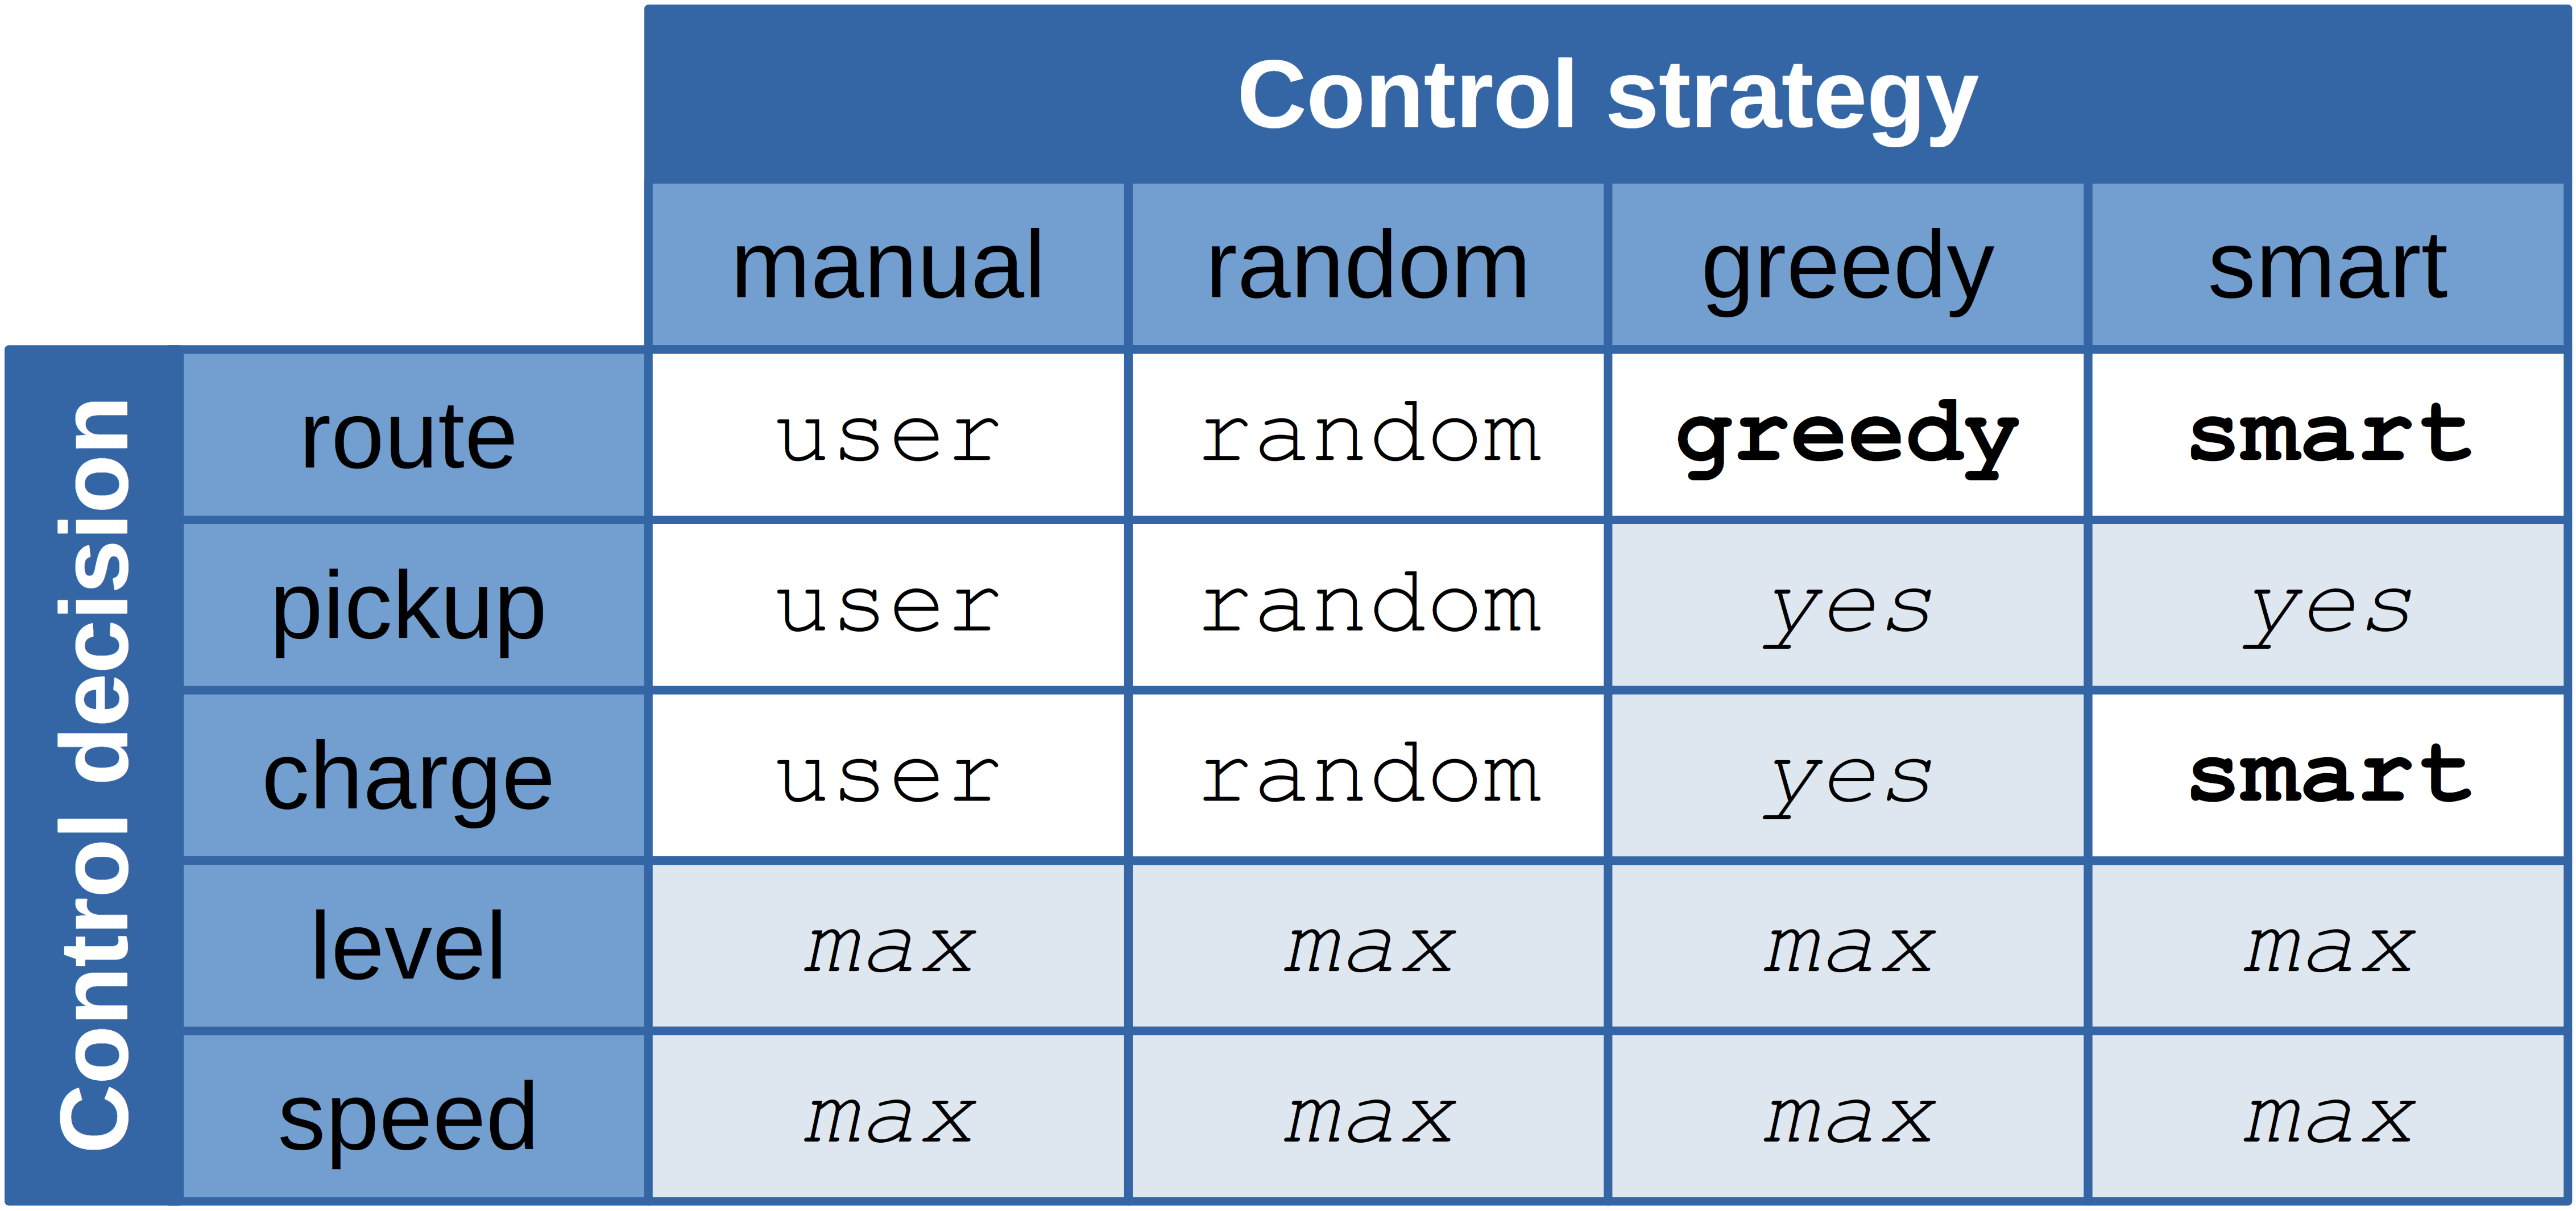
\includegraphics[width=0.8\columnwidth]{control_strategy_overview.png}
    \caption{Overview of the control strategies.}
    \label{fig:control-strategies}
\end{figure}

In the following, we describe the logics behind each of the control strategies in more detail.

\subsubsection*{Manual control strategy}
\label{sec:controller-manual}

The manual control strategy delegates routing, demand pickup, and charge decisions to the tool user using input dialogs.
The remaining control decisions are derived automatically.

Figure~\ref{fig:manual-controller-route} shows the input dialog for routing decisions, which pops up when a vehicle arrives a an intersection.
The dialog provides the name of the vehicle (\texttt{V} in the example) as well as the possible follow-up road segments (\texttt{C->D} and \texttt{C->E} in the example).
Note that \texttt{C}, \texttt{D}, and \texttt{E} represent the names of the intersections connected through the segments.
The user can select the desired routing option by pressing the button for the respective follow-up segment.

\begin{figure}[!ht]
    \centering
    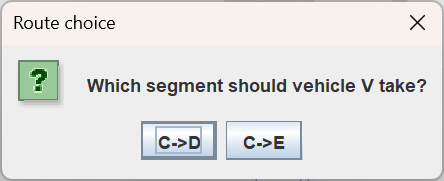
\includegraphics[scale=0.4]{../../screenshots/manual-controller-route.png}
    \caption{Route choice.}
    \label{fig:manual-controller-route}
\end{figure}

Figure~\ref{fig:manual-controller-demand} shows the input dialog for demand pickup decisions, which pops up when a vehicle arrives at the pickup location of an appeared and unserved demand.
The dialog provides the name of the vehicle (\texttt{U} in the example), the data of the demand (i.e.\ the pickup location and earliest pickup time as well as the dropoff location and latest dropoff time), and the two choice buttons (i.e.\ yes and no).

\begin{figure}[!ht]
    \centering
    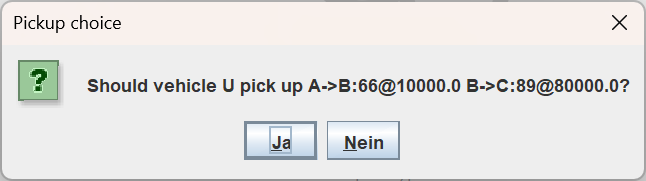
\includegraphics[scale=0.4]{../../screenshots/manual-controller-demand.png}
    \caption{Pickup choice.}
    \label{fig:manual-controller-demand}
\end{figure}

Figure~\ref{fig:manual-controller-charge} shows the input dialog for vehicle charging decisions, which pops up when a vehicle arrives at the location of an unoccupied charging station.
The dialog provides the name of the vehicle (\texttt{U} in the example), the location of the charging station (\texttt{A->B:50} in the example), and the buttons for the two available choices (i.e.\ yes and no).

\begin{figure}[!ht]
    \centering
    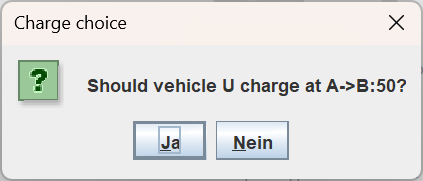
\includegraphics[scale=0.4]{../../screenshots/manual-controller-charge.png}
    \caption{Charge choice.}
    \label{fig:manual-controller-charge}
\end{figure}

Finally, the strategy always selects the maximum driving speed for each vehicle without considering possible collisions.
And the strategy always chooses to fully charge the battery of each vehicle after the user decided to start the charging process.

\subsubsection*{Random control strategy}
\label{sec:controller-random}

The random control strategy uses a standard random number generator for making the routing, demand pickup, and charging decisions described previously.
For each decision, the strategy assigns equal probabilities to the available choices (i.e.\ outgoing segments of an intersection or yes and no).
Furthermore, driving speed and target battery charge level are handled equally to the manual controller described in the previous section.

\subsubsection*{Greedy control strategy}
\label{sec:controller-greedy}

The greedy control strategy uses a more sophisticated logic for determining routing decisions upon arrivals of vehicles at intersections of the driving infrastructure.
The logic comprises four rules, which are processed in sequential order until one rule applies:
\begin{enumerate}
    \item When the battery of the vehicle is only half full or less, the strategy randomly selects an outgoing road segment with charging station if such segment is avaiable.
    \item Then, when the vehicle carries one or more demands, the strategy randomly selects the drop-off segment of one such demand if reachable directly via the intersection.
    \item Next, when the vehicle carries no demand, the strategy randomly selects the pick-up segment of an unserved demand if reachable directly via the intersection.
    \item Finaly, when none of the above three rules apply, the strategy randomly selects any of the outgoing road segments of the current intersection with uniform probability distribution.
\end{enumerate}
Note that the above rules of the routing logic only consider the next segment and do not perform a look-ahead across more segments.
Finally, the greedy control strategy always chooses to pick up demands or charge vehicle batteries if arriving at an unserved demand pick-up location or charging station.
Also, the strategy always chooses to drive at maximum speed and to fully charge the batteries if a charging process has started.

\subsubsection*{Smart control strategy}
\label{sec:controller-smart}

The smart control strategy uses an even more sophisticated strategy for determining routing decisions upon intersection arrivals of vehicles.
The logic again comprises four rules, which are processed in sequential order until one rule applies:
\begin{enumerate}
    \item When the vehicle carries one ore more demands and a charging station can be reached via their drop-off location with the current battery level, the closest such demand is selected.
    \item When the vehicle does not carry any demands and a charging station can be reached via the pick-up location of an unserved demand, the closest such demand is selected for pick-up.
    \item When the vehicle carries no demands and does not plan to pick-up a new demand, the segment leading to the closest charging station is selected if reachable with the remaining battery level.
    \item Finally, when none of the above three rules apply, again the strategy randomly selects any of the outgoing road segments of the current intersection with uniform probability distribution.
\end{enumerate}
When arriving at an unused charing station, the smart control strategy only starts charging if no other charging station can be reached with the current battery level.
Furthermore, when the charging station is used, but not other charging station can be reached, the strategy lets the vehicle wait at the station to become free.
Finally, with this strategy vehicles always pick up unassigned demands when passing by, charge their batteries fully when at a charging station, and drive with maximum speed.

\subsection{Data recorder}
\label{sec:statistics-interface}

During simulation, a number of events are recorded for visualization of system (and control strategy) performance as well as further processing such as strategy training.
Figure~\ref{fig:statistics-interface} shows the provided methods of the data recorder interface.

\begin{figure}[!ht]
    \centering
    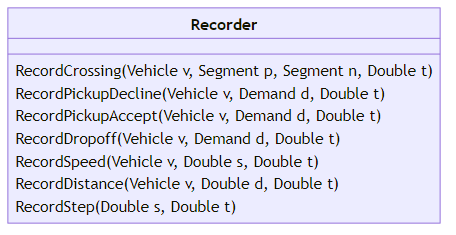
\includegraphics[scale=0.4]{../../diagrams/statistics/classes-v2.png}
    \caption{Statistics interface.}
    \label{fig:statistics-interface}
\end{figure}

The recorder tracks, when a vehicle crosses an intersection, and records the associated routing decision of the control strategy.
Then, the recorder tracks, when a vehicle passes by an unassigned demand and the control strategy declines or accepts the pick up.
Similarly, the recorder tracks, when a vehicle drops off a demand at its target location.
Furthermore, the recorder continuously tracks the speed and the overall travel distance of the vehicles.
Finally, the recorder also tracks the size of the time steps made during discrete event simulation.

Currently, we use the data about intersection crossing for determining bottlenecks in the driving infrastructure.
Also, we use the data about pick ups and drop offs for determining per demand waiting and driving as well as delays.
In the future, we plan to add more recording capabilities as well as exploring additional use cases for the data.

\subsection{Simulation engine}
\label{sec:simulation-engine}

As explained previously, the simulation engine is responsible for computing the events, delegating control decisions, updating the system state, and sending data to the recorder.
\begin{enumerate}
    \item Update vehicle segment (including routing decision)
    \item Disconnect vehicle from charging station (if full or controller decision)
    \item Connect vehicle to charging station (if not full and controller decision)
    \item Pick up demand (if controller decision)
    \item Drop off demand
    \item Drop off demand (empty battery)
    \item Update vehicle speed (including speed decision)
\end{enumerate}
Compute time of the next event
\begin{itemize}
    \item Speed selection timeout (controller decision)
    \item Charge speed update or charging station disconnect timeout (controller decision)
    \item Battery level exhaustion timeout
    \item Segment end timeout / intersection arrival timeout
    \item Demand appearance timeout (mainly for visualization)
    \item Demand overdue timeout (mainly for visualization)
    \item Charging station arrival timeout
    \item Battery full timeout
    \item Demand pick up arrival timeout
    \item Demand drop off arrival timeout
    \item Vehicle attach/detach timeout
\end{itemize}
Update battery level and location of vehicle.
Record traveled distance and time step.
Detect collision

\subsection{Specific applications}
\label{sec:application}

Based on the previous components we implemented two specific applications:
The first application can be used for comparing the performance of different control strategies (see Section~\ref{sec:controller-comparison}).
The second application can be used for comparing the performance of different driving and charging infrastructures as well as fleet configurations (see Section~\ref{sec:infrastructure-comparison}).

\subsubsection{Control strategy comparison}
\label{sec:controller-comparison}

To compare control strategies, we apply the strategies to the same system configuration (including driving and charging infrastructure as well as vehicle fleets) and scenario (i.e.\ demand profile).
For performance evaluation, we currently measure the times between demand appearance at the pick up location and disappearance at the drop off location.
Figure~\ref{fig:controller-comparison} shows an example system configuration, on which the random, the greedy, and the smart control strategy are applied.

\begin{figure}[!ht]
    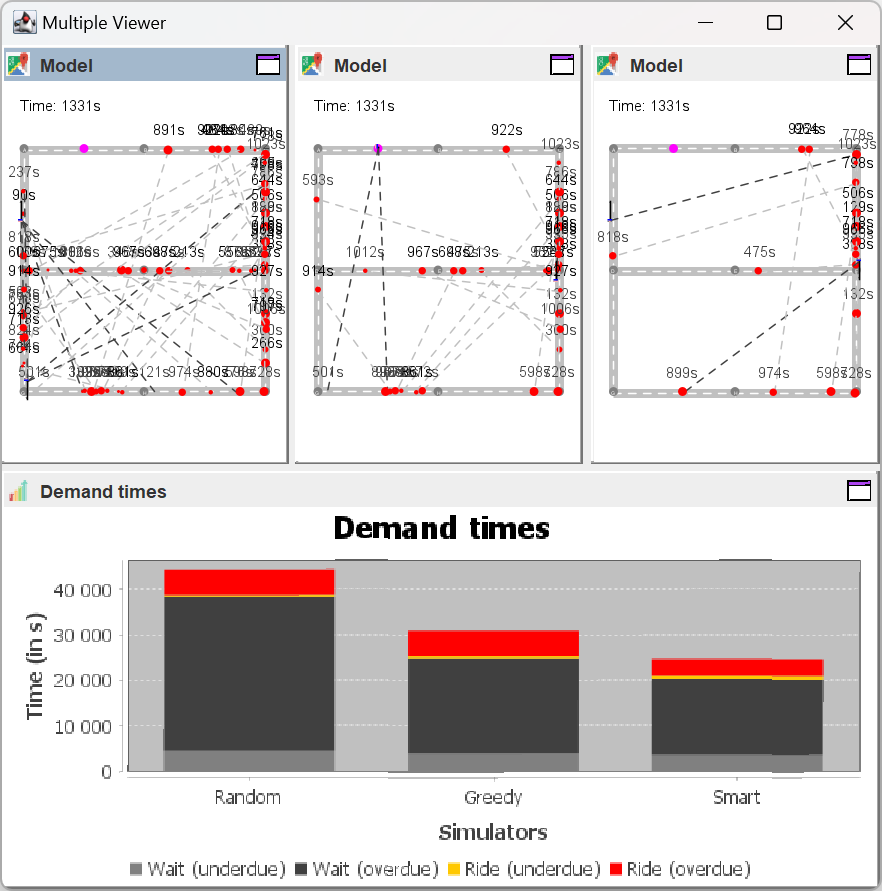
\includegraphics[width=\columnwidth]{controller_comparison.png}
    \caption{Controller comparison.}
    \label{fig:controller-comparison}
\end{figure}

The upper part of the window shows for each control strategy the current system state including the vehicle locations and the active demands.
The lower part of the window shows for each control strategy the total times between demand appearance and disappearance.
From the diagram we can deduct that in this simulation run the smart control strategy showed superior performance over the others.
Note that due to the random nature of the control strategies, the result might have been very different.

\subsubsection{System configuration comparison}
\label{sec:infrastructure-comparison}

To compare system configurations, we instead apply the same control strategy and scenario (i.e.\ demand profile) to different versions of the driving and charging infrastructure as well as the fleet configuration.
Note that different versions of the driving infrastructure might include additional road segments not present in other versions.
Hence, we require that demands only reference road segments, which are included in every version of the driving infrastructure.
Figure~\ref{fig:infratructure-comparison} shows an example, where the smart control strategy is applied to different infrastructure stages.

\begin{figure}[!ht]
    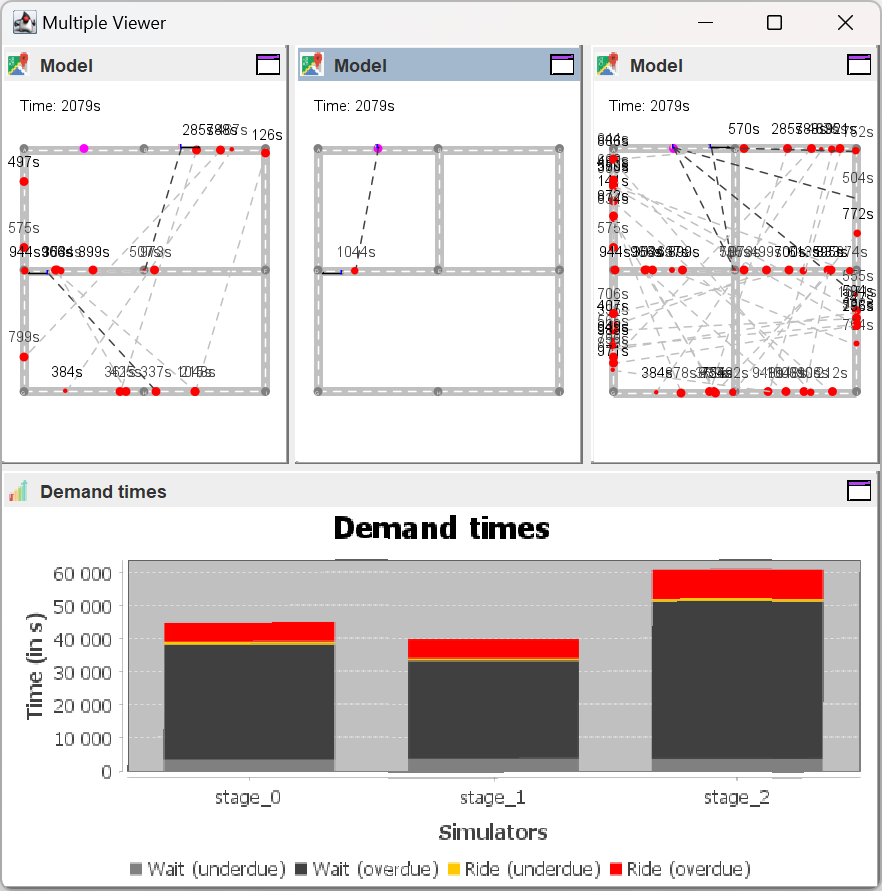
\includegraphics[width=\columnwidth]{infrastructure_comparison.png}
    \caption{Infrastructure comparison.}
    \label{fig:infratructure-comparison}
\end{figure}

Again, the upper part of the window shows for each control strategy the current system state including vehicle locations and demands.
Also, the lower part of the window shows for each system configuration the total times between demand appearance and disappearance.
In this simulation run, the system configuration in the middle, which adds only one additional road segment, has the best performance.
This example mainly shows, that the smart control strategy not always delivers optimal results, which is necessary for a fair comparison of infrastructures.

\section{Conclusion}
\label{sec:conclusion}

\textcolor{red}{TODO}

\bibliographystyle{plain}
\bibliography{main}

\end{document}
